\documentclass[1p]{elsarticle_modified}
%\bibliographystyle{elsarticle-num}

%\usepackage[colorlinks]{hyperref}
%\usepackage{abbrmath_seonhwa} %\Abb, \Ascr, \Acal ,\Abf, \Afrak
\usepackage{amsfonts}
\usepackage{amssymb}
\usepackage{amsmath}
\usepackage{amsthm}
\usepackage{scalefnt}
\usepackage{amsbsy}
\usepackage{kotex}
\usepackage{caption}
\usepackage{subfig}
\usepackage{color}
\usepackage{graphicx}
\usepackage{xcolor} %% white, black, red, green, blue, cyan, magenta, yellow
\usepackage{float}
\usepackage{setspace}
\usepackage{hyperref}

\usepackage{tikz}
\usetikzlibrary{arrows}

\usepackage{multirow}
\usepackage{array} % fixed length table
\usepackage{hhline}

%%%%%%%%%%%%%%%%%%%%%
\makeatletter
\renewcommand*\env@matrix[1][\arraystretch]{%
	\edef\arraystretch{#1}%
	\hskip -\arraycolsep
	\let\@ifnextchar\new@ifnextchar
	\array{*\c@MaxMatrixCols c}}
\makeatother %https://tex.stackexchange.com/questions/14071/how-can-i-increase-the-line-spacing-in-a-matrix
%%%%%%%%%%%%%%%

\usepackage[normalem]{ulem}

\newcommand{\msout}[1]{\ifmmode\text{\sout{\ensuremath{#1}}}\else\sout{#1}\fi}
%SOURCE: \msout is \stkout macro in https://tex.stackexchange.com/questions/20609/strikeout-in-math-mode

\newcommand{\cancel}[1]{
	\ifmmode
	{\color{red}\msout{#1}}
	\else
	{\color{red}\sout{#1}}
	\fi
}

\newcommand{\add}[1]{
	{\color{blue}\uwave{#1}}
}

\newcommand{\replace}[2]{
	\ifmmode
	{\color{red}\msout{#1}}{\color{blue}\uwave{#2}}
	\else
	{\color{red}\sout{#1}}{\color{blue}\uwave{#2}}
	\fi
}

\newcommand{\Sol}{\mathcal{S}} %segment
\newcommand{\D}{D} %diagram
\newcommand{\A}{\mathcal{A}} %arc


%%%%%%%%%%%%%%%%%%%%%%%%%%%%%5 test

\def\sl{\operatorname{\textup{SL}}(2,\Cbb)}
\def\psl{\operatorname{\textup{PSL}}(2,\Cbb)}
\def\quan{\mkern 1mu \triangleright \mkern 1mu}

\theoremstyle{definition}
\newtheorem{thm}{Theorem}[section]
\newtheorem{prop}[thm]{Proposition}
\newtheorem{lem}[thm]{Lemma}
\newtheorem{ques}[thm]{Question}
\newtheorem{cor}[thm]{Corollary}
\newtheorem{defn}[thm]{Definition}
\newtheorem{exam}[thm]{Example}
\newtheorem{rmk}[thm]{Remark}
\newtheorem{alg}[thm]{Algorithm}

\newcommand{\I}{\sqrt{-1}}
\begin{document}

%\begin{frontmatter}
%
%\title{Boundary parabolic representations of knots up to 8 crossings}
%
%%% Group authors per affiliation:
%\author{Yunhi Cho} 
%\address{Department of Mathematics, University of Seoul, Seoul, Korea}
%\ead{yhcho@uos.ac.kr}
%
%
%\author{Seonhwa Kim} %\fnref{s_kim}}
%\address{Center for Geometry and Physics, Institute for Basic Science, Pohang, 37673, Korea}
%\ead{ryeona17@ibs.re.kr}
%
%\author{Hyuk Kim}
%\address{Department of Mathematical Sciences, Seoul National University, Seoul 08826, Korea}
%\ead{hyukkim@snu.ac.kr}
%
%\author{Seokbeom Yoon}
%\address{Department of Mathematical Sciences, Seoul National University, Seoul, 08826,  Korea}
%\ead{sbyoon15@snu.ac.kr}
%
%\begin{abstract}
%We find all boundary parabolic representation of knots up to 8 crossings.
%
%\end{abstract}
%\begin{keyword}
%    \MSC[2010] 57M25 
%\end{keyword}
%
%\end{frontmatter}

%\linenumbers
%\tableofcontents
%
\newcommand\colored[1]{\textcolor{white}{\rule[-0.35ex]{0.8em}{1.4ex}}\kern-0.8em\color{red} #1}%
%\newcommand\colored[1]{\textcolor{white}{ #1}\kern-2.17ex	\textcolor{white}{ #1}\kern-1.81ex	\textcolor{white}{ #1}\kern-2.15ex\color{red}#1	}

{\Large $\underline{11a_{316}~(K11a_{316})}$}

\setlength{\tabcolsep}{10pt}
\renewcommand{\arraystretch}{1.6}
\vspace{1cm}\begin{tabular}{m{100pt}>{\centering\arraybackslash}m{274pt}}
\multirow{5}{120pt}{
	\centering
	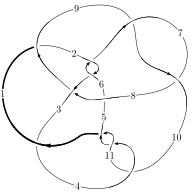
\includegraphics[width=112pt]{../../../GIT/diagram.site/Diagrams/png/565_11a_316.png}\\
\ \ \ A knot diagram\footnotemark}&
\allowdisplaybreaks
\textbf{Linearized knot diagam} \\
\cline{2-2}
 &
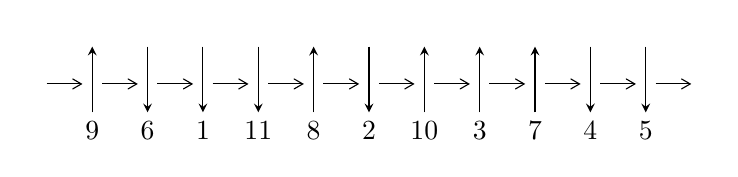
\begin{tikzpicture}[x=20pt, y=17pt]
	% nodes
	\node (C0) at (0, 0) {};
	\node (C1) at (1, 0) {};
	\node (C1U) at (1, +1) {};
	\node (C1D) at (1, -1) {9};

	\node (C2) at (2, 0) {};
	\node (C2U) at (2, +1) {};
	\node (C2D) at (2, -1) {6};

	\node (C3) at (3, 0) {};
	\node (C3U) at (3, +1) {};
	\node (C3D) at (3, -1) {1};

	\node (C4) at (4, 0) {};
	\node (C4U) at (4, +1) {};
	\node (C4D) at (4, -1) {11};

	\node (C5) at (5, 0) {};
	\node (C5U) at (5, +1) {};
	\node (C5D) at (5, -1) {8};

	\node (C6) at (6, 0) {};
	\node (C6U) at (6, +1) {};
	\node (C6D) at (6, -1) {2};

	\node (C7) at (7, 0) {};
	\node (C7U) at (7, +1) {};
	\node (C7D) at (7, -1) {10};

	\node (C8) at (8, 0) {};
	\node (C8U) at (8, +1) {};
	\node (C8D) at (8, -1) {3};

	\node (C9) at (9, 0) {};
	\node (C9U) at (9, +1) {};
	\node (C9D) at (9, -1) {7};

	\node (C10) at (10, 0) {};
	\node (C10U) at (10, +1) {};
	\node (C10D) at (10, -1) {4};

	\node (C11) at (11, 0) {};
	\node (C11U) at (11, +1) {};
	\node (C11D) at (11, -1) {5};
	\node (C12) at (12, 0) {};

	% arrows
	\draw[->,>={angle 60}]
	(C0) edge (C1) (C1) edge (C2) (C2) edge (C3) (C3) edge (C4) (C4) edge (C5) (C5) edge (C6) (C6) edge (C7) (C7) edge (C8) (C8) edge (C9) (C9) edge (C10) (C10) edge (C11) (C11) edge (C12) ;	\draw[->,>=stealth]
	(C1D) edge (C1U) (C2U) edge (C2D) (C3U) edge (C3D) (C4U) edge (C4D) (C5D) edge (C5U) (C6U) edge (C6D) (C7D) edge (C7U) (C8D) edge (C8U) (C9D) edge (C9U) (C10U) edge (C10D) (C11U) edge (C11D) ;
	\end{tikzpicture} \\
\hhline{~~} \\& 
\textbf{Solving Sequence} \\ \cline{2-2} 
 &
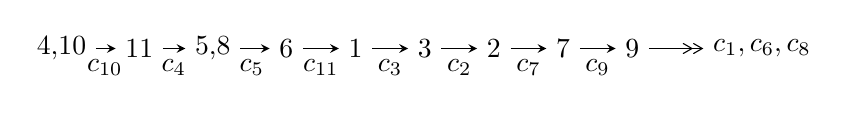
\begin{tikzpicture}[x=25pt, y=7pt]
	% node
	\node (A0) at (-1/8, 0) {4,10};
	\node (A1) at (1, 0) {11};
	\node (A2) at (33/16, 0) {5,8};
	\node (A3) at (25/8, 0) {6};
	\node (A4) at (33/8, 0) {1};
	\node (A5) at (41/8, 0) {3};
	\node (A6) at (49/8, 0) {2};
	\node (A7) at (57/8, 0) {7};
	\node (A8) at (65/8, 0) {9};
	\node (C1) at (1/2, -1) {$c_{10}$};
	\node (C2) at (3/2, -1) {$c_{4}$};
	\node (C3) at (21/8, -1) {$c_{5}$};
	\node (C4) at (29/8, -1) {$c_{11}$};
	\node (C5) at (37/8, -1) {$c_{3}$};
	\node (C6) at (45/8, -1) {$c_{2}$};
	\node (C7) at (53/8, -1) {$c_{7}$};
	\node (C8) at (61/8, -1) {$c_{9}$};
	\node (A9) at (10, 0) {$c_{1},c_{6},c_{8}$};

	% edge
	\draw[->,>=stealth]	
	(A0) edge (A1) (A1) edge (A2) (A2) edge (A3) (A3) edge (A4) (A4) edge (A5) (A5) edge (A6) (A6) edge (A7) (A7) edge (A8) ;
	\draw[->>,>={angle 60}]	
	(A8) edge (A9);
\end{tikzpicture} \\ 

\end{tabular} \\

\footnotetext{
The image of knot diagram is generated by the software ``\textbf{Draw programme}" developed by Andrew Bartholomew(\url{http://www.layer8.co.uk/maths/draw/index.htm\#Running-draw}), where we modified some parts for our purpose(\url{https://github.com/CATsTAILs/LinksPainter}).
}\phantom \\ \newline 
\centering \textbf{Ideals for irreducible components\footnotemark of $X_{\text{par}}$} 
 
\begin{align*}
I^u_{1}&=\langle 
1.80623\times10^{32} u^{61}-5.14761\times10^{32} u^{60}+\cdots+4.61017\times10^{32} b-1.10416\times10^{32},\\
\phantom{I^u_{1}}&\phantom{= \langle  }-6.91332\times10^{32} u^{61}-7.53652\times10^{32} u^{60}+\cdots+2.30509\times10^{33} a-2.31132\times10^{33},\;u^{62}-2 u^{61}+\cdots+3 u+1\rangle \\
I^u_{2}&=\langle 
b-1,\;5 a+u-2,\;u^2+u-1\rangle \\
\\
\end{align*}
\raggedright * 2 irreducible components of $\dim_{\mathbb{C}}=0$, with total 64 representations.\\
\footnotetext{All coefficients of polynomials are rational numbers. But the coefficients are sometimes approximated in decimal forms when there is not enough margin.}
\newpage
\renewcommand{\arraystretch}{1}
\centering \section*{I. $I^u_{1}= \langle 1.81\times10^{32} u^{61}-5.15\times10^{32} u^{60}+\cdots+4.61\times10^{32} b-1.10\times10^{32},\;-6.91\times10^{32} u^{61}-7.54\times10^{32} u^{60}+\cdots+2.31\times10^{33} a-2.31\times10^{33},\;u^{62}-2 u^{61}+\cdots+3 u+1 \rangle$}
\flushleft \textbf{(i) Arc colorings}\\
\begin{tabular}{m{7pt} m{180pt} m{7pt} m{180pt} }
\flushright $a_{4}=$&$\begin{pmatrix}0\\u\end{pmatrix}$ \\
\flushright $a_{10}=$&$\begin{pmatrix}1\\0\end{pmatrix}$ \\
\flushright $a_{11}=$&$\begin{pmatrix}1\\u^2\end{pmatrix}$ \\
\flushright $a_{5}=$&$\begin{pmatrix}- u\\- u^3+u\end{pmatrix}$ \\
\flushright $a_{8}=$&$\begin{pmatrix}0.299916 u^{61}+0.326952 u^{60}+\cdots-3.67552 u+1.00270\\-0.391793 u^{61}+1.11658 u^{60}+\cdots-0.782541 u+0.239505\end{pmatrix}$ \\
\flushright $a_{6}=$&$\begin{pmatrix}-1.37364 u^{61}+0.955447 u^{60}+\cdots+15.8721 u+3.35880\\0.226500 u^{61}-0.438184 u^{60}+\cdots+5.26406 u+0.574836\end{pmatrix}$ \\
\flushright $a_{1}=$&$\begin{pmatrix}- u^2+1\\- u^4+2 u^2\end{pmatrix}$ \\
\flushright $a_{3}=$&$\begin{pmatrix}u^5-2 u^3+u\\u^7-3 u^5+2 u^3+u\end{pmatrix}$ \\
\flushright $a_{2}=$&$\begin{pmatrix}0.403303 u^{61}+1.11034 u^{60}+\cdots+3.59385 u-1.62323\\0.435823 u^{61}-0.0545467 u^{60}+\cdots-0.0437745 u-1.01330\end{pmatrix}$ \\
\flushright $a_{7}=$&$\begin{pmatrix}0.691708 u^{61}-0.789625 u^{60}+\cdots-2.89298 u+0.763197\\-0.391793 u^{61}+1.11658 u^{60}+\cdots-0.782541 u+0.239505\end{pmatrix}$ \\
\flushright $a_{9}=$&$\begin{pmatrix}0.210043 u^{61}+0.259417 u^{60}+\cdots-3.20318 u+1.25041\\-0.348888 u^{61}+0.656606 u^{60}+\cdots+0.331553 u+0.825406\end{pmatrix}$\\ \flushright $a_{9}=$&$\begin{pmatrix}0.210043 u^{61}+0.259417 u^{60}+\cdots-3.20318 u+1.25041\\-0.348888 u^{61}+0.656606 u^{60}+\cdots+0.331553 u+0.825406\end{pmatrix}$\\&\end{tabular}
\flushleft \textbf{(ii) Obstruction class $= -1$}\\~\\
\flushleft \textbf{(iii) Cusp Shapes $= 3.89183 u^{61}-9.68250 u^{60}+\cdots-4.68341 u+13.0328$}\\~\\
\newpage\renewcommand{\arraystretch}{1}
\flushleft \textbf{(iv) u-Polynomials at the component}\newline \\
\begin{tabular}{m{50pt}|m{274pt}}
Crossings & \hspace{64pt}u-Polynomials at each crossing \\
\hline $$\begin{aligned}c_{1}\end{aligned}$$&$\begin{aligned}
&5(5 u^{62}+7 u^{61}+\cdots+100038 u-28017)
\end{aligned}$\\
\hline $$\begin{aligned}c_{2},c_{6}\end{aligned}$$&$\begin{aligned}
&u^{62}+2 u^{61}+\cdots- u+1
\end{aligned}$\\
\hline $$\begin{aligned}c_{3}\end{aligned}$$&$\begin{aligned}
&u^{62}-6 u^{61}+\cdots+795 u-117
\end{aligned}$\\
\hline $$\begin{aligned}c_{4},c_{10},c_{11}\end{aligned}$$&$\begin{aligned}
&u^{62}+2 u^{61}+\cdots-3 u+1
\end{aligned}$\\
\hline $$\begin{aligned}c_{5}\end{aligned}$$&$\begin{aligned}
&5(5 u^{62}-14 u^{61}+\cdots+61755 u+8377)
\end{aligned}$\\
\hline $$\begin{aligned}c_{7},c_{9}\end{aligned}$$&$\begin{aligned}
&u^{62}+3 u^{61}+\cdots+214 u-25
\end{aligned}$\\
\hline $$\begin{aligned}c_{8}\end{aligned}$$&$\begin{aligned}
&u^{62}+u^{61}+\cdots+280 u-100
\end{aligned}$\\
\hline
\end{tabular}\\~\\
\newpage\renewcommand{\arraystretch}{1}
\flushleft \textbf{(v) Riley Polynomials at the component}\newline \\
\begin{tabular}{m{50pt}|m{274pt}}
Crossings & \hspace{64pt}Riley Polynomials at each crossing \\
\hline $$\begin{aligned}c_{1}\end{aligned}$$&$\begin{aligned}
&25(25 y^{62}-1309 y^{61}+\cdots-1.54576\times10^{10} y+7.84952\times10^{8})
\end{aligned}$\\
\hline $$\begin{aligned}c_{2},c_{6}\end{aligned}$$&$\begin{aligned}
&y^{62}+42 y^{61}+\cdots-25 y+1
\end{aligned}$\\
\hline $$\begin{aligned}c_{3}\end{aligned}$$&$\begin{aligned}
&y^{62}+18 y^{61}+\cdots-440613 y+13689
\end{aligned}$\\
\hline $$\begin{aligned}c_{4},c_{10},c_{11}\end{aligned}$$&$\begin{aligned}
&y^{62}-54 y^{61}+\cdots-25 y+1
\end{aligned}$\\
\hline $$\begin{aligned}c_{5}\end{aligned}$$&$\begin{aligned}
&25(25 y^{62}-286 y^{61}+\cdots-1.29244\times10^{9} y+7.01741\times10^{7})
\end{aligned}$\\
\hline $$\begin{aligned}c_{7},c_{9}\end{aligned}$$&$\begin{aligned}
&y^{62}-49 y^{61}+\cdots-22596 y+625
\end{aligned}$\\
\hline $$\begin{aligned}c_{8}\end{aligned}$$&$\begin{aligned}
&y^{62}-15 y^{61}+\cdots-413000 y+10000
\end{aligned}$\\
\hline
\end{tabular}\\~\\
\newpage\flushleft \textbf{(vi) Complex Volumes and Cusp Shapes}
$$\begin{array}{c|c|c}  
\text{Solutions to }I^u_{1}& \I (\text{vol} + \sqrt{-1}CS) & \text{Cusp shape}\\
 \hline 
\begin{aligned}
u &= -0.887619 + 0.514849 I \\
a &= -0.168834 - 0.676664 I \\
b &= -1.351070 - 0.186432 I\end{aligned}
 & \phantom{-}6.81266 + 5.56177 I & \phantom{-}4.66163 - 5.86539 I \\ \hline\begin{aligned}
u &= -0.887619 - 0.514849 I \\
a &= -0.168834 + 0.676664 I \\
b &= -1.351070 + 0.186432 I\end{aligned}
 & \phantom{-}6.81266 - 5.56177 I & \phantom{-}4.66163 + 5.86539 I \\ \hline\begin{aligned}
u &= -0.956988 + 0.457534 I \\
a &= -0.411794 - 0.142908 I \\
b &= -1.44265 + 0.39962 I\end{aligned}
 & \phantom{-}7.18631 - 7.01551 I & \phantom{-0.000000 } 0 \\ \hline\begin{aligned}
u &= -0.956988 - 0.457534 I \\
a &= -0.411794 + 0.142908 I \\
b &= -1.44265 - 0.39962 I\end{aligned}
 & \phantom{-}7.18631 + 7.01551 I & \phantom{-0.000000 } 0 \\ \hline\begin{aligned}
u &= -0.268927 + 0.858943 I \\
a &= \phantom{-}0.487450 - 0.791896 I \\
b &= -1.326860 + 0.042366 I\end{aligned}
 & \phantom{-}8.77447 - 0.73219 I & \phantom{-}8.26642 + 0.24787 I \\ \hline\begin{aligned}
u &= -0.268927 - 0.858943 I \\
a &= \phantom{-}0.487450 + 0.791896 I \\
b &= -1.326860 - 0.042366 I\end{aligned}
 & \phantom{-}8.77447 + 0.73219 I & \phantom{-}8.26642 - 0.24787 I \\ \hline\begin{aligned}
u &= \phantom{-}0.981110 + 0.511433 I \\
a &= -0.156001 + 0.318273 I \\
b &= -1.245360 - 0.167604 I\end{aligned}
 & \phantom{-}2.26101 + 1.03760 I & \phantom{-0.000000 } 0 \\ \hline\begin{aligned}
u &= \phantom{-}0.981110 - 0.511433 I \\
a &= -0.156001 - 0.318273 I \\
b &= -1.245360 + 0.167604 I\end{aligned}
 & \phantom{-}2.26101 - 1.03760 I & \phantom{-0.000000 } 0 \\ \hline\begin{aligned}
u &= \phantom{-}0.216176 + 0.854810 I \\
a &= \phantom{-}0.879762 + 0.839368 I \\
b &= -1.284170 + 0.305083 I\end{aligned}
 & \phantom{-}4.62237 - 5.84398 I & \phantom{-}3.48358 + 6.22366 I \\ \hline\begin{aligned}
u &= \phantom{-}0.216176 - 0.854810 I \\
a &= \phantom{-}0.879762 - 0.839368 I \\
b &= -1.284170 - 0.305083 I\end{aligned}
 & \phantom{-}4.62237 + 5.84398 I & \phantom{-}3.48358 - 6.22366 I\\
 \hline 
 \end{array}$$\newpage$$\begin{array}{c|c|c}  
\text{Solutions to }I^u_{1}& \I (\text{vol} + \sqrt{-1}CS) & \text{Cusp shape}\\
 \hline 
\begin{aligned}
u &= -0.222629 + 0.830394 I \\
a &= \phantom{-}0.97517 - 1.10506 I \\
b &= -1.47365 - 0.48988 I\end{aligned}
 & \phantom{-}9.4690 + 11.6120 I & \phantom{-}5.02297 - 7.15875 I \\ \hline\begin{aligned}
u &= -0.222629 - 0.830394 I \\
a &= \phantom{-}0.97517 + 1.10506 I \\
b &= -1.47365 + 0.48988 I\end{aligned}
 & \phantom{-}9.4690 - 11.6120 I & \phantom{-}5.02297 + 7.15875 I \\ \hline\begin{aligned}
u &= -1.133930 + 0.168026 I \\
a &= \phantom{-}1.26618 - 0.92935 I \\
b &= \phantom{-}0.586572 - 1.058950 I\end{aligned}
 & \phantom{-}1.22471 - 2.22328 I & \phantom{-0.000000 } 0 \\ \hline\begin{aligned}
u &= -1.133930 - 0.168026 I \\
a &= \phantom{-}1.26618 + 0.92935 I \\
b &= \phantom{-}0.586572 + 1.058950 I\end{aligned}
 & \phantom{-}1.22471 + 2.22328 I & \phantom{-0.000000 } 0 \\ \hline\begin{aligned}
u &= \phantom{-}1.233700 + 0.140829 I \\
a &= \phantom{-}1.11356 + 0.95442 I \\
b &= \phantom{-}0.498573 + 0.517622 I\end{aligned}
 & -2.34840 - 0.48442 I & \phantom{-0.000000 } 0 \\ \hline\begin{aligned}
u &= \phantom{-}1.233700 - 0.140829 I \\
a &= \phantom{-}1.11356 - 0.95442 I \\
b &= \phantom{-}0.498573 - 0.517622 I\end{aligned}
 & -2.34840 + 0.48442 I & \phantom{-0.000000 } 0 \\ \hline\begin{aligned}
u &= \phantom{-}1.228560 + 0.275128 I \\
a &= \phantom{-}1.155710 - 0.633770 I \\
b &= \phantom{-}1.77170 + 0.45104 I\end{aligned}
 & \phantom{-}4.49072 - 1.35832 I & \phantom{-0.000000 } 0 \\ \hline\begin{aligned}
u &= \phantom{-}1.228560 - 0.275128 I \\
a &= \phantom{-}1.155710 + 0.633770 I \\
b &= \phantom{-}1.77170 - 0.45104 I\end{aligned}
 & \phantom{-}4.49072 + 1.35832 I & \phantom{-0.000000 } 0 \\ \hline\begin{aligned}
u &= -0.154976 + 0.717888 I \\
a &= -0.542160 + 0.195736 I \\
b &= \phantom{-}0.278710 + 1.257500 I\end{aligned}
 & \phantom{-}3.96361 + 5.62230 I & \phantom{-}4.59110 - 7.16807 I \\ \hline\begin{aligned}
u &= -0.154976 - 0.717888 I \\
a &= -0.542160 - 0.195736 I \\
b &= \phantom{-}0.278710 - 1.257500 I\end{aligned}
 & \phantom{-}3.96361 - 5.62230 I & \phantom{-}4.59110 + 7.16807 I\\
 \hline 
 \end{array}$$\newpage$$\begin{array}{c|c|c}  
\text{Solutions to }I^u_{1}& \I (\text{vol} + \sqrt{-1}CS) & \text{Cusp shape}\\
 \hline 
\begin{aligned}
u &= \phantom{-}0.046542 + 0.724748 I \\
a &= -1.208990 - 0.366912 I \\
b &= \phantom{-}1.66460 - 0.64188 I\end{aligned}
 & \phantom{-}8.09797 - 2.26515 I & \phantom{-}10.09980 + 3.27421 I \\ \hline\begin{aligned}
u &= \phantom{-}0.046542 - 0.724748 I \\
a &= -1.208990 + 0.366912 I \\
b &= \phantom{-}1.66460 + 0.64188 I\end{aligned}
 & \phantom{-}8.09797 + 2.26515 I & \phantom{-}10.09980 - 3.27421 I \\ \hline\begin{aligned}
u &= -1.263000 + 0.236260 I \\
a &= -0.487348 + 0.065309 I \\
b &= \phantom{-}1.210290 - 0.144045 I\end{aligned}
 & -0.11388 + 2.17095 I & \phantom{-0.000000 } 0 \\ \hline\begin{aligned}
u &= -1.263000 - 0.236260 I \\
a &= -0.487348 - 0.065309 I \\
b &= \phantom{-}1.210290 + 0.144045 I\end{aligned}
 & -0.11388 - 2.17095 I & \phantom{-0.000000 } 0 \\ \hline\begin{aligned}
u &= -1.288710 + 0.185153 I \\
a &= \phantom{-}2.28058 - 2.74209 I \\
b &= \phantom{-}0.864085 + 0.005366 I\end{aligned}
 & \phantom{-}0.03983 + 2.79266 I & \phantom{-0.000000 } 0 \\ \hline\begin{aligned}
u &= -1.288710 - 0.185153 I \\
a &= \phantom{-}2.28058 + 2.74209 I \\
b &= \phantom{-}0.864085 - 0.005366 I\end{aligned}
 & \phantom{-}0.03983 - 2.79266 I & \phantom{-0.000000 } 0 \\ \hline\begin{aligned}
u &= \phantom{-}0.179463 + 0.661396 I \\
a &= -0.055951 - 0.244113 I \\
b &= \phantom{-}0.050410 - 0.678849 I\end{aligned}
 & \phantom{-}0.49280 - 2.22863 I & -1.88873 + 4.27642 I \\ \hline\begin{aligned}
u &= \phantom{-}0.179463 - 0.661396 I \\
a &= -0.055951 + 0.244113 I \\
b &= \phantom{-}0.050410 + 0.678849 I\end{aligned}
 & \phantom{-}0.49280 + 2.22863 I & -1.88873 - 4.27642 I \\ \hline\begin{aligned}
u &= -1.293980 + 0.298379 I \\
a &= \phantom{-}0.30932 + 2.31869 I \\
b &= \phantom{-}1.60267 + 0.81560 I\end{aligned}
 & \phantom{-}3.91657 + 5.96640 I & \phantom{-0.000000 } 0 \\ \hline\begin{aligned}
u &= -1.293980 - 0.298379 I \\
a &= \phantom{-}0.30932 - 2.31869 I \\
b &= \phantom{-}1.60267 - 0.81560 I\end{aligned}
 & \phantom{-}3.91657 - 5.96640 I & \phantom{-0.000000 } 0\\
 \hline 
 \end{array}$$\newpage$$\begin{array}{c|c|c}  
\text{Solutions to }I^u_{1}& \I (\text{vol} + \sqrt{-1}CS) & \text{Cusp shape}\\
 \hline 
\begin{aligned}
u &= \phantom{-}1.301670 + 0.265672 I \\
a &= -0.14106 - 2.23111 I \\
b &= \phantom{-}1.118260 - 0.376395 I\end{aligned}
 & -0.57816 - 4.41700 I & \phantom{-0.000000 } 0 \\ \hline\begin{aligned}
u &= \phantom{-}1.301670 - 0.265672 I \\
a &= -0.14106 + 2.23111 I \\
b &= \phantom{-}1.118260 + 0.376395 I\end{aligned}
 & -0.57816 + 4.41700 I & \phantom{-0.000000 } 0 \\ \hline\begin{aligned}
u &= -0.042843 + 0.662429 I \\
a &= -1.81923 + 1.14582 I \\
b &= \phantom{-}1.139070 + 0.251694 I\end{aligned}
 & \phantom{-}3.63336 + 1.04794 I & \phantom{-}2.34672 - 0.35139 I \\ \hline\begin{aligned}
u &= -0.042843 - 0.662429 I \\
a &= -1.81923 - 1.14582 I \\
b &= \phantom{-}1.139070 - 0.251694 I\end{aligned}
 & \phantom{-}3.63336 - 1.04794 I & \phantom{-}2.34672 + 0.35139 I \\ \hline\begin{aligned}
u &= \phantom{-}1.334310 + 0.246440 I \\
a &= \phantom{-}1.069770 - 0.893080 I \\
b &= \phantom{-}0.231740 - 0.094385 I\end{aligned}
 & -1.00664 - 2.96825 I & \phantom{-0.000000 } 0 \\ \hline\begin{aligned}
u &= \phantom{-}1.334310 - 0.246440 I \\
a &= \phantom{-}1.069770 + 0.893080 I \\
b &= \phantom{-}0.231740 + 0.094385 I\end{aligned}
 & -1.00664 + 2.96825 I & \phantom{-0.000000 } 0 \\ \hline\begin{aligned}
u &= -0.115133 + 0.619794 I \\
a &= \phantom{-}1.22726 + 1.09164 I \\
b &= \phantom{-}0.413434 - 0.098972 I\end{aligned}
 & \phantom{-}3.55015 - 0.20409 I & \phantom{-}5.98628 - 1.19975 I \\ \hline\begin{aligned}
u &= -0.115133 - 0.619794 I \\
a &= \phantom{-}1.22726 - 1.09164 I \\
b &= \phantom{-}0.413434 + 0.098972 I\end{aligned}
 & \phantom{-}3.55015 + 0.20409 I & \phantom{-}5.98628 + 1.19975 I \\ \hline\begin{aligned}
u &= \phantom{-}1.372160 + 0.035845 I \\
a &= \phantom{-}0.47764 + 1.70860 I \\
b &= -0.237289 + 0.862746 I\end{aligned}
 & -4.26849 + 2.33228 I & \phantom{-0.000000 } 0 \\ \hline\begin{aligned}
u &= \phantom{-}1.372160 - 0.035845 I \\
a &= \phantom{-}0.47764 - 1.70860 I \\
b &= -0.237289 - 0.862746 I\end{aligned}
 & -4.26849 - 2.33228 I & \phantom{-0.000000 } 0\\
 \hline 
 \end{array}$$\newpage$$\begin{array}{c|c|c}  
\text{Solutions to }I^u_{1}& \I (\text{vol} + \sqrt{-1}CS) & \text{Cusp shape}\\
 \hline 
\begin{aligned}
u &= \phantom{-}1.354390 + 0.299440 I \\
a &= -0.88402 - 1.77945 I \\
b &= \phantom{-}0.150670 - 1.364490 I\end{aligned}
 & -0.80126 - 9.32026 I & \phantom{-0.000000 } 0 \\ \hline\begin{aligned}
u &= \phantom{-}1.354390 - 0.299440 I \\
a &= -0.88402 + 1.77945 I \\
b &= \phantom{-}0.150670 + 1.364490 I\end{aligned}
 & -0.80126 + 9.32026 I & \phantom{-0.000000 } 0 \\ \hline\begin{aligned}
u &= -1.364120 + 0.277183 I \\
a &= -0.491592 + 1.171990 I \\
b &= -0.043760 + 0.847969 I\end{aligned}
 & -4.39333 + 5.67407 I & \phantom{-0.000000 } 0 \\ \hline\begin{aligned}
u &= -1.364120 - 0.277183 I \\
a &= -0.491592 - 1.171990 I \\
b &= -0.043760 - 0.847969 I\end{aligned}
 & -4.39333 - 5.67407 I & \phantom{-0.000000 } 0 \\ \hline\begin{aligned}
u &= -1.41802 + 0.08070 I \\
a &= -0.165441 - 1.216540 I \\
b &= -0.566676 - 0.567301 I\end{aligned}
 & -7.01139 + 2.01626 I & \phantom{-0.000000 } 0 \\ \hline\begin{aligned}
u &= -1.41802 - 0.08070 I \\
a &= -0.165441 + 1.216540 I \\
b &= -0.566676 + 0.567301 I\end{aligned}
 & -7.01139 - 2.01626 I & \phantom{-0.000000 } 0 \\ \hline\begin{aligned}
u &= \phantom{-}1.39937 + 0.34656 I \\
a &= -0.28769 + 2.13431 I \\
b &= -1.47028 + 0.55396 I\end{aligned}
 & \phantom{-}4.3271 - 15.8582 I & \phantom{-0.000000 } 0 \\ \hline\begin{aligned}
u &= \phantom{-}1.39937 - 0.34656 I \\
a &= -0.28769 - 2.13431 I \\
b &= -1.47028 - 0.55396 I\end{aligned}
 & \phantom{-}4.3271 + 15.8582 I & \phantom{-0.000000 } 0 \\ \hline\begin{aligned}
u &= -1.39672 + 0.35868 I \\
a &= -0.16352 - 1.69873 I \\
b &= -1.286260 - 0.404733 I\end{aligned}
 & -0.48145 + 10.21060 I & \phantom{-0.000000 } 0 \\ \hline\begin{aligned}
u &= -1.39672 - 0.35868 I \\
a &= -0.16352 + 1.69873 I \\
b &= -1.286260 + 0.404733 I\end{aligned}
 & -0.48145 - 10.21060 I & \phantom{-0.000000 } 0\\
 \hline 
 \end{array}$$\newpage$$\begin{array}{c|c|c}  
\text{Solutions to }I^u_{1}& \I (\text{vol} + \sqrt{-1}CS) & \text{Cusp shape}\\
 \hline 
\begin{aligned}
u &= \phantom{-}0.463287 + 0.297906 I \\
a &= \phantom{-}0.788454 + 0.539829 I \\
b &= -0.250407 + 0.311008 I\end{aligned}
 & -1.008560 - 0.666322 I & -7.37810 + 3.95165 I \\ \hline\begin{aligned}
u &= \phantom{-}0.463287 - 0.297906 I \\
a &= \phantom{-}0.788454 - 0.539829 I \\
b &= -0.250407 - 0.311008 I\end{aligned}
 & -1.008560 + 0.666322 I & -7.37810 - 3.95165 I \\ \hline\begin{aligned}
u &= -0.550158 + 0.016824 I \\
a &= \phantom{-}1.33228 + 1.00368 I \\
b &= \phantom{-}0.256229 + 0.735207 I\end{aligned}
 & \phantom{-}1.45921 + 2.58594 I & -1.55168 - 3.98149 I \\ \hline\begin{aligned}
u &= -0.550158 - 0.016824 I \\
a &= \phantom{-}1.33228 - 1.00368 I \\
b &= \phantom{-}0.256229 - 0.735207 I\end{aligned}
 & \phantom{-}1.45921 - 2.58594 I & -1.55168 + 3.98149 I \\ \hline\begin{aligned}
u &= \phantom{-}1.42814 + 0.36734 I \\
a &= -0.564087 + 1.146080 I \\
b &= -1.270380 + 0.067319 I\end{aligned}
 & \phantom{-}3.38499 - 3.70672 I & \phantom{-0.000000 } 0 \\ \hline\begin{aligned}
u &= \phantom{-}1.42814 - 0.36734 I \\
a &= -0.564087 - 1.146080 I \\
b &= -1.270380 - 0.067319 I\end{aligned}
 & \phantom{-}3.38499 + 3.70672 I & \phantom{-0.000000 } 0 \\ \hline\begin{aligned}
u &= \phantom{-}1.50001 + 0.04160 I \\
a &= -1.29195 + 0.81714 I \\
b &= -1.205330 + 0.382950 I\end{aligned}
 & -1.16526 - 6.77623 I & \phantom{-0.000000 } 0 \\ \hline\begin{aligned}
u &= \phantom{-}1.50001 - 0.04160 I \\
a &= -1.29195 - 0.81714 I \\
b &= -1.205330 - 0.382950 I\end{aligned}
 & -1.16526 + 6.77623 I & \phantom{-0.000000 } 0 \\ \hline\begin{aligned}
u &= \phantom{-}0.239018 + 0.279647 I \\
a &= \phantom{-}3.12607 - 0.97399 I \\
b &= \phantom{-}1.190070 - 0.194532 I\end{aligned}
 & \phantom{-}4.30759 - 0.97665 I & -0.516718 + 1.197110 I \\ \hline\begin{aligned}
u &= \phantom{-}0.239018 - 0.279647 I \\
a &= \phantom{-}3.12607 + 0.97399 I \\
b &= \phantom{-}1.190070 + 0.194532 I\end{aligned}
 & \phantom{-}4.30759 + 0.97665 I & -0.516718 - 1.197110 I\\
 \hline 
 \end{array}$$\newpage$$\begin{array}{c|c|c}  
\text{Solutions to }I^u_{1}& \I (\text{vol} + \sqrt{-1}CS) & \text{Cusp shape}\\
 \hline 
\begin{aligned}
u &= -1.63921\phantom{ +0.000000I} \\
a &= -0.771484\phantom{ +0.000000I} \\
b &= -1.04713\phantom{ +0.000000I}\end{aligned}
 & -7.12923\phantom{ +0.000000I} & \phantom{-0.000000 } 0 \\ \hline\begin{aligned}
u &= -0.201088\phantom{ +0.000000I} \\
a &= \phantom{-}2.67242\phantom{ +0.000000I} \\
b &= \phantom{-}0.901231\phantom{ +0.000000I}\end{aligned}
 & \phantom{-}1.30954\phantom{ +0.000000I} & \phantom{-}9.93960\phantom{ +0.000000I}\\
 \hline 
 \end{array}$$\newpage\newpage\renewcommand{\arraystretch}{1}
\centering \section*{II. $I^u_{2}= \langle b-1,\;5 a+u-2,\;u^2+u-1 \rangle$}
\flushleft \textbf{(i) Arc colorings}\\
\begin{tabular}{m{7pt} m{180pt} m{7pt} m{180pt} }
\flushright $a_{4}=$&$\begin{pmatrix}0\\u\end{pmatrix}$ \\
\flushright $a_{10}=$&$\begin{pmatrix}1\\0\end{pmatrix}$ \\
\flushright $a_{11}=$&$\begin{pmatrix}1\\- u+1\end{pmatrix}$ \\
\flushright $a_{5}=$&$\begin{pmatrix}- u\\- u+1\end{pmatrix}$ \\
\flushright $a_{8}=$&$\begin{pmatrix}-\frac{1}{5} u+\frac{2}{5}\\1\end{pmatrix}$ \\
\flushright $a_{6}=$&$\begin{pmatrix}- u+\frac{1}{5}\\-\frac{4}{5} u+\frac{8}{5}\end{pmatrix}$ \\
\flushright $a_{1}=$&$\begin{pmatrix}u\\u\end{pmatrix}$ \\
\flushright $a_{3}=$&$\begin{pmatrix}2 u-1\\3 u-1\end{pmatrix}$ \\
\flushright $a_{2}=$&$\begin{pmatrix}\frac{4}{5} u\\\frac{3}{5} u-\frac{1}{5}\end{pmatrix}$ \\
\flushright $a_{7}=$&$\begin{pmatrix}-\frac{1}{5} u-\frac{3}{5}\\1\end{pmatrix}$ \\
\flushright $a_{9}=$&$\begin{pmatrix}-\frac{1}{5} u+\frac{2}{5}\\1\end{pmatrix}$\\ \flushright $a_{9}=$&$\begin{pmatrix}-\frac{1}{5} u+\frac{2}{5}\\1\end{pmatrix}$\\&\end{tabular}
\flushleft \textbf{(ii) Obstruction class $= 1$}\\~\\
\flushleft \textbf{(iii) Cusp Shapes $= \frac{72}{5} u-13$}\\~\\
\newpage\renewcommand{\arraystretch}{1}
\flushleft \textbf{(iv) u-Polynomials at the component}\newline \\
\begin{tabular}{m{50pt}|m{274pt}}
Crossings & \hspace{64pt}u-Polynomials at each crossing \\
\hline $$\begin{aligned}c_{1}\end{aligned}$$&$\begin{aligned}
&5(5 u^2-1)
\end{aligned}$\\
\hline $$\begin{aligned}c_{2},c_{10},c_{11}\end{aligned}$$&$\begin{aligned}
&u^2+u-1
\end{aligned}$\\
\hline $$\begin{aligned}c_{3}\end{aligned}$$&$\begin{aligned}
&u^2+3 u+1
\end{aligned}$\\
\hline $$\begin{aligned}c_{4},c_{6}\end{aligned}$$&$\begin{aligned}
&u^2- u-1
\end{aligned}$\\
\hline $$\begin{aligned}c_{5}\end{aligned}$$&$\begin{aligned}
&5(5 u^2+5 u+1)
\end{aligned}$\\
\hline $$\begin{aligned}c_{7}\end{aligned}$$&$\begin{aligned}
&(u+1)^2
\end{aligned}$\\
\hline $$\begin{aligned}c_{8}\end{aligned}$$&$\begin{aligned}
&u^2
\end{aligned}$\\
\hline $$\begin{aligned}c_{9}\end{aligned}$$&$\begin{aligned}
&(u-1)^2
\end{aligned}$\\
\hline
\end{tabular}\\~\\
\newpage\renewcommand{\arraystretch}{1}
\flushleft \textbf{(v) Riley Polynomials at the component}\newline \\
\begin{tabular}{m{50pt}|m{274pt}}
Crossings & \hspace{64pt}Riley Polynomials at each crossing \\
\hline $$\begin{aligned}c_{1}\end{aligned}$$&$\begin{aligned}
&25(5 y-1)^2
\end{aligned}$\\
\hline $$\begin{aligned}c_{2},c_{4},c_{6}\\c_{10},c_{11}\end{aligned}$$&$\begin{aligned}
&y^2-3 y+1
\end{aligned}$\\
\hline $$\begin{aligned}c_{3}\end{aligned}$$&$\begin{aligned}
&y^2-7 y+1
\end{aligned}$\\
\hline $$\begin{aligned}c_{5}\end{aligned}$$&$\begin{aligned}
&25(25 y^2-15 y+1)
\end{aligned}$\\
\hline $$\begin{aligned}c_{7},c_{9}\end{aligned}$$&$\begin{aligned}
&(y-1)^2
\end{aligned}$\\
\hline $$\begin{aligned}c_{8}\end{aligned}$$&$\begin{aligned}
&y^2
\end{aligned}$\\
\hline
\end{tabular}\\~\\
\newpage\flushleft \textbf{(vi) Complex Volumes and Cusp Shapes}
$$\begin{array}{c|c|c}  
\text{Solutions to }I^u_{2}& \I (\text{vol} + \sqrt{-1}CS) & \text{Cusp shape}\\
 \hline 
\begin{aligned}
u &= \phantom{-}0.618034\phantom{ +0.000000I} \\
a &= \phantom{-}0.276393\phantom{ +0.000000I} \\
b &= \phantom{-}1.00000\phantom{ +0.000000I}\end{aligned}
 & \phantom{-}0.657974\phantom{ +0.000000I} & -4.10030\phantom{ +0.000000I} \\ \hline\begin{aligned}
u &= -1.61803\phantom{ +0.000000I} \\
a &= \phantom{-}0.723607\phantom{ +0.000000I} \\
b &= \phantom{-}1.00000\phantom{ +0.000000I}\end{aligned}
 & -7.23771\phantom{ +0.000000I} & -36.3000\phantom{ +0.000000I}\\
 \hline 
 \end{array}$$\newpage
\newpage\renewcommand{\arraystretch}{1}
\centering \section*{ III. u-Polynomials}
\begin{tabular}{m{50pt}|m{274pt}}
Crossings & \hspace{64pt}u-Polynomials at each crossing \\
\hline $$\begin{aligned}c_{1}\end{aligned}$$&$\begin{aligned}
&25(5 u^2-1)(5 u^{62}+7 u^{61}+\cdots+100038 u-28017)
\end{aligned}$\\
\hline $$\begin{aligned}c_{2}\end{aligned}$$&$\begin{aligned}
&(u^2+u-1)(u^{62}+2 u^{61}+\cdots- u+1)
\end{aligned}$\\
\hline $$\begin{aligned}c_{3}\end{aligned}$$&$\begin{aligned}
&(u^2+3 u+1)(u^{62}-6 u^{61}+\cdots+795 u-117)
\end{aligned}$\\
\hline $$\begin{aligned}c_{4}\end{aligned}$$&$\begin{aligned}
&(u^2- u-1)(u^{62}+2 u^{61}+\cdots-3 u+1)
\end{aligned}$\\
\hline $$\begin{aligned}c_{5}\end{aligned}$$&$\begin{aligned}
&25(5 u^2+5 u+1)(5 u^{62}-14 u^{61}+\cdots+61755 u+8377)
\end{aligned}$\\
\hline $$\begin{aligned}c_{6}\end{aligned}$$&$\begin{aligned}
&(u^2- u-1)(u^{62}+2 u^{61}+\cdots- u+1)
\end{aligned}$\\
\hline $$\begin{aligned}c_{7}\end{aligned}$$&$\begin{aligned}
&((u+1)^2)(u^{62}+3 u^{61}+\cdots+214 u-25)
\end{aligned}$\\
\hline $$\begin{aligned}c_{8}\end{aligned}$$&$\begin{aligned}
&u^2(u^{62}+u^{61}+\cdots+280 u-100)
\end{aligned}$\\
\hline $$\begin{aligned}c_{9}\end{aligned}$$&$\begin{aligned}
&((u-1)^2)(u^{62}+3 u^{61}+\cdots+214 u-25)
\end{aligned}$\\
\hline $$\begin{aligned}c_{10},c_{11}\end{aligned}$$&$\begin{aligned}
&(u^2+u-1)(u^{62}+2 u^{61}+\cdots-3 u+1)
\end{aligned}$\\
\hline
\end{tabular}\newpage\renewcommand{\arraystretch}{1}
\centering \section*{ IV. Riley Polynomials}
\begin{tabular}{m{50pt}|m{274pt}}
Crossings & \hspace{64pt}Riley Polynomials at each crossing \\
\hline $$\begin{aligned}c_{1}\end{aligned}$$&$\begin{aligned}
&625(5 y-1)^2\\
&\cdot(25 y^{62}-1309 y^{61}+\cdots-15457580352 y+784952289)
\end{aligned}$\\
\hline $$\begin{aligned}c_{2},c_{6}\end{aligned}$$&$\begin{aligned}
&(y^2-3 y+1)(y^{62}+42 y^{61}+\cdots-25 y+1)
\end{aligned}$\\
\hline $$\begin{aligned}c_{3}\end{aligned}$$&$\begin{aligned}
&(y^2-7 y+1)(y^{62}+18 y^{61}+\cdots-440613 y+13689)
\end{aligned}$\\
\hline $$\begin{aligned}c_{4},c_{10},c_{11}\end{aligned}$$&$\begin{aligned}
&(y^2-3 y+1)(y^{62}-54 y^{61}+\cdots-25 y+1)
\end{aligned}$\\
\hline $$\begin{aligned}c_{5}\end{aligned}$$&$\begin{aligned}
&625(25 y^2-15 y+1)\\
&\cdot(25 y^{62}-286 y^{61}+\cdots-1292437581 y+70174129)
\end{aligned}$\\
\hline $$\begin{aligned}c_{7},c_{9}\end{aligned}$$&$\begin{aligned}
&((y-1)^2)(y^{62}-49 y^{61}+\cdots-22596 y+625)
\end{aligned}$\\
\hline $$\begin{aligned}c_{8}\end{aligned}$$&$\begin{aligned}
&y^2(y^{62}-15 y^{61}+\cdots-413000 y+10000)
\end{aligned}$\\
\hline
\end{tabular}
\vskip 2pc
\end{document}